\pagebreak
\section{Vehicle Tests - Steering - Linear Area for \si{K_p}} \label{app:LinearAreaKp}
\textbf{Name: Group 510}\\
\textbf{Date: 30/09 - 2015}

\subsubsection{Purpose}
The purpose of this test is to find a minimum and maximum values that could be used for the steering proportional controller's gain, \si{K_p}.

\subsubsection{Setup}
The setup is the same as in the steering gain test, see \appref{app:steeringGainTest}.

\subsubsection{List of Equipment}

\begin{table}[H]
\begin{tabular}{|p{10cm}|p{4cm}|}
\hline%------------------------------------------------------------------------------------
  \textbf{Instrument}                     &  \textbf{Type}       \\
\hline%------------------------------------------------------------------------------------
  Computer                                &  Acer C720p    \\
\hline %-----------------------------------------------------------------------------------
\end{tabular}
\end{table}

\subsubsection{Procedure}

\begin{enumerate}
  \item Disconnect the battery.
  \item Connect the Arduino to the computer.
  \item Upload the test code to the Arduino board using the Arduino IDE  \cite{ArduinoIDE}.
  \item Switch the vehicle's power on.
  \item Open a serial terminal via PuTTY \cite{PuTTY} immediately after plugging the battery.
  \item Wait two seconds, then follow the vehicle with the connected computer.
  \item Wait until the vehicle stops before ending the measurements by unplugging the connected computer from the Arduino.
  \item Shut the vehicle's power off.
  \item Redo the test multiples while increasing the wanted controller gain.
  \item Plot the angle of the vehicle using Matlab.
\end{enumerate}

\subsubsection{Results}

In this test, instead of changing the velocity between tests, the proportional controller's gain is changing from 1 to 4 with a step of 0,5.\\

\begin{figure}[H]
  \centering
  %Trim margins @:   left        bottom       right       top
  \adjustbox{ trim = {.15\width} {.30\height} {.15\width} {.30\height}, clip }
  {
    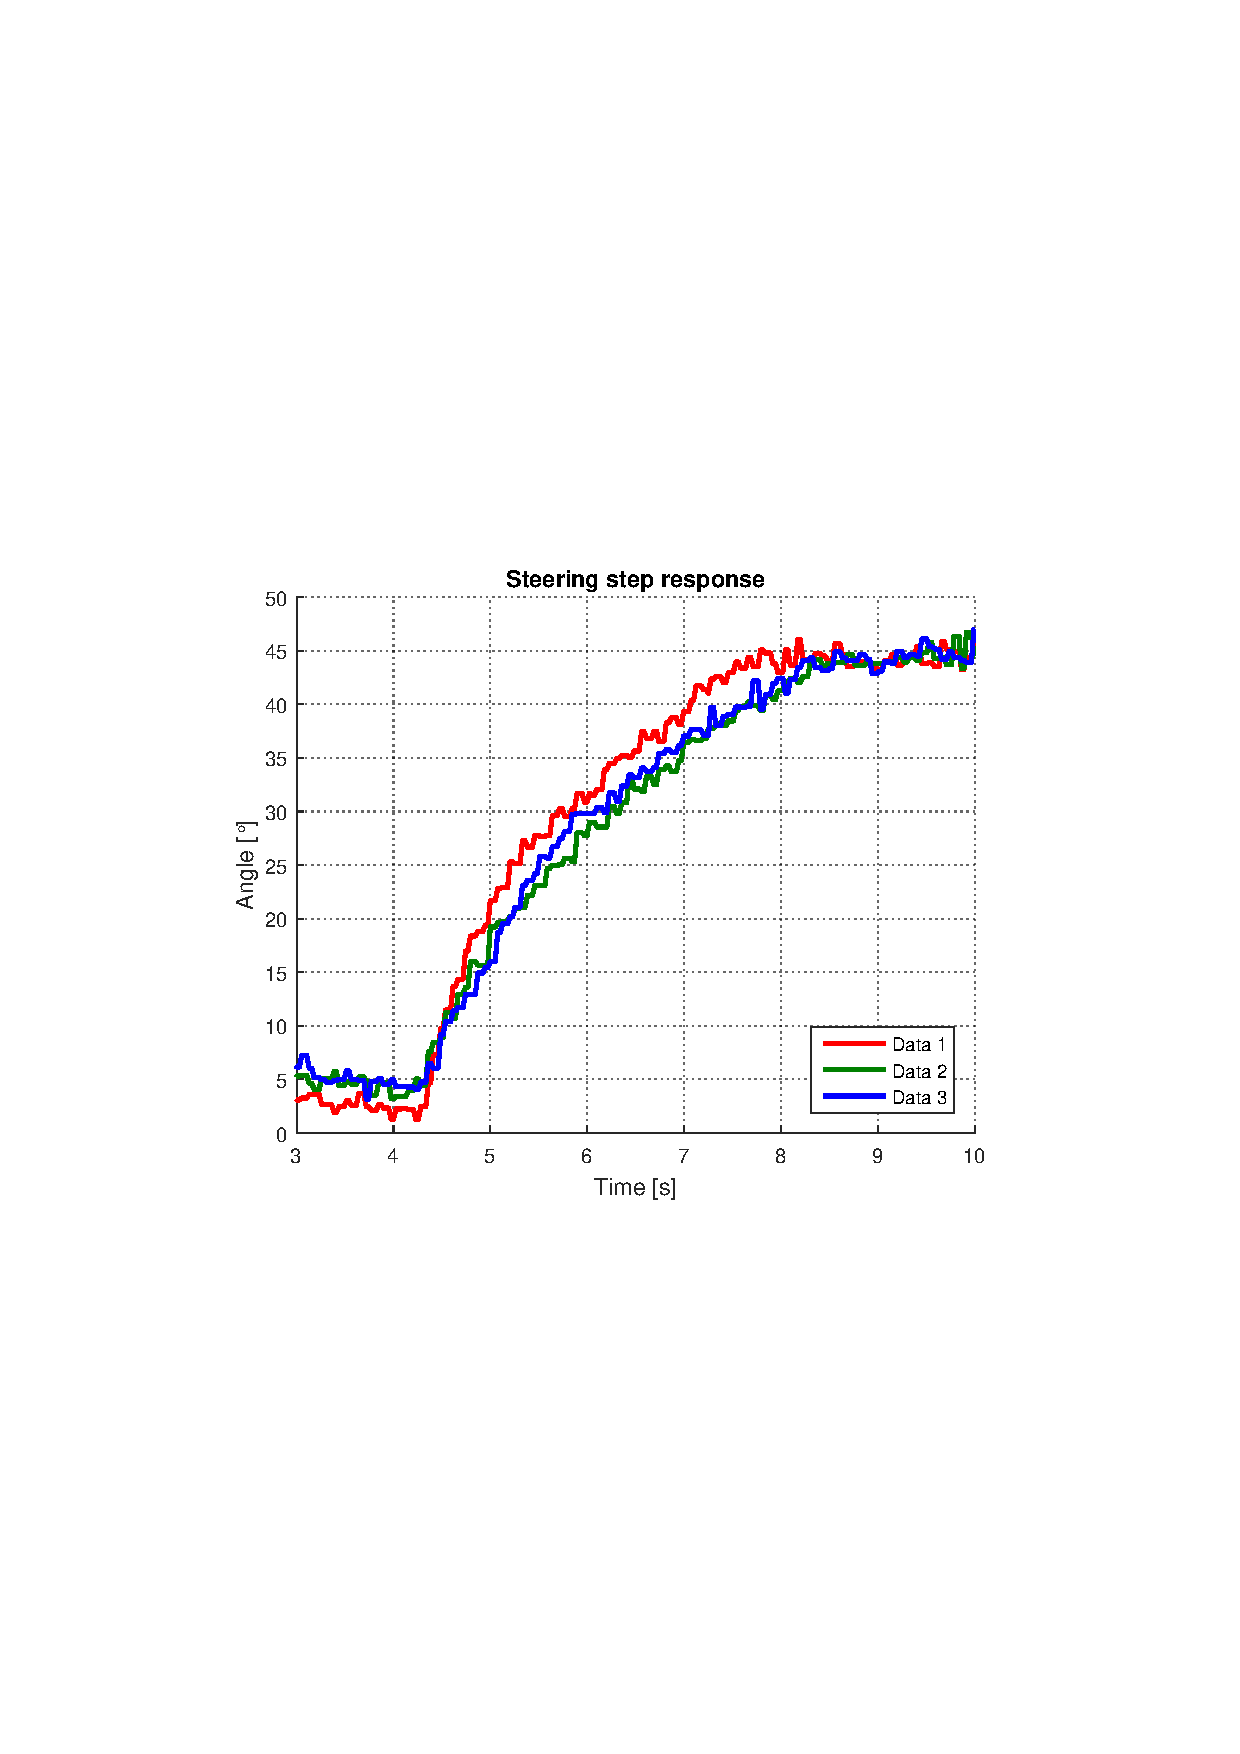
\includegraphics[width=1.2\textwidth]{figures/steeringStep_P2.pdf}
  }
  \caption{Plot of three test where the vehicle is turning, where the x-axis is time and the y-axis is angle.}
  \label{fig:steeringAngleVsTimeKvKp}
\end{figure}
%
By utilizing 18 measurements, of which three are illustrated in \figref{fig:steeringAngleVsTimeKvKp}, 18 time-constants are found on the graph. The corresponding values for the steering gain, \si{K_{steering}}, are calculated by using the formula from \eqref{SteeringTimeconstant}, see \tableref{tab:steeringGains}.

Given the fact that the velocity should be maintained constant, the steering gain, \si{K_{steering}} should remain the same as long as the proportional controller's gain, \si{K_p} is within the right range. Outside this particular area, the steering might become non-linear and this should therefore be avoided as much as possible to simplify the controlling the process.
%
\begin{table}[H]
\begin{tabular}{|p{2cm}|p{2cm}|p{3cm}|p{2cm}|p{2cm}|p{3cm}|}
\hline%-----------------------------------------------------------------------------------------------------------------
\textbf{Test no.}  &  \textbf{\si{K_p}} &  \textbf{\si{K_{steering}}}  &  \textbf{Test no.}   &  \textbf{\si{K_p}}  &    \textbf{\si{K_{steering}}}        \\
\hline%-----------------------------------------------------------------------------------------------------------------
           1    &   1   &   0.180831826   &   10    &     2.5    &           0.344827586              \\
\hline%-----------------------------------------------------------------------------------------------------------------
           2    &   1   &   0.180342651   &  11    &      2.5    &        0.294117647                 \\
\hline%-----------------------------------------------------------------------------------------------------------------
           3    &   1   &    0.17088175   &  12    &       2.5     &           0.291970803              \\
\hline%-----------------------------------------------------------------------------------------------------------------
           4    &   1.5 &   0.266666667   &   13   &       3     &         0.362318841                \\
\hline%-----------------------------------------------------------------------------------------------------------------
           5    &   1.5 &   0.259403372   &   14   &        3    &         0.256410256                \\
\hline%-----------------------------------------------------------------------------------------------------------------
           6    &   1.5 &   0.254452926   &    15    &       3.5     &          0.840336134               \\
\hline%-----------------------------------------------------------------------------------------------------------------
           7    &   2   &  0.265957447    &   16    &          3.5     &            0.549450549             \\
\hline%-----------------------------------------------------------------------------------------------------------------
           8    &   2   &   0.284090909   &    17   &            3.5     &           0.476190476              \\
\hline%-----------------------------------------------------------------------------------------------------------------
           9    &   2   &   0.37037037    &    18    &           4       &         0.549450549                \\
\hline%-----------------------------------------------------------------------------------------------------------------
\end{tabular}
\caption{Steering gains calculated from the tests}
\label{tab:steeringGains}
\end{table}

\begin{figure}[H]
  \centering
  %Trim margins @:   left        bottom       right       top
  \adjustbox{ trim = {.15\width} {.30\height} {.15\width} {.30\height}, clip }
  {
    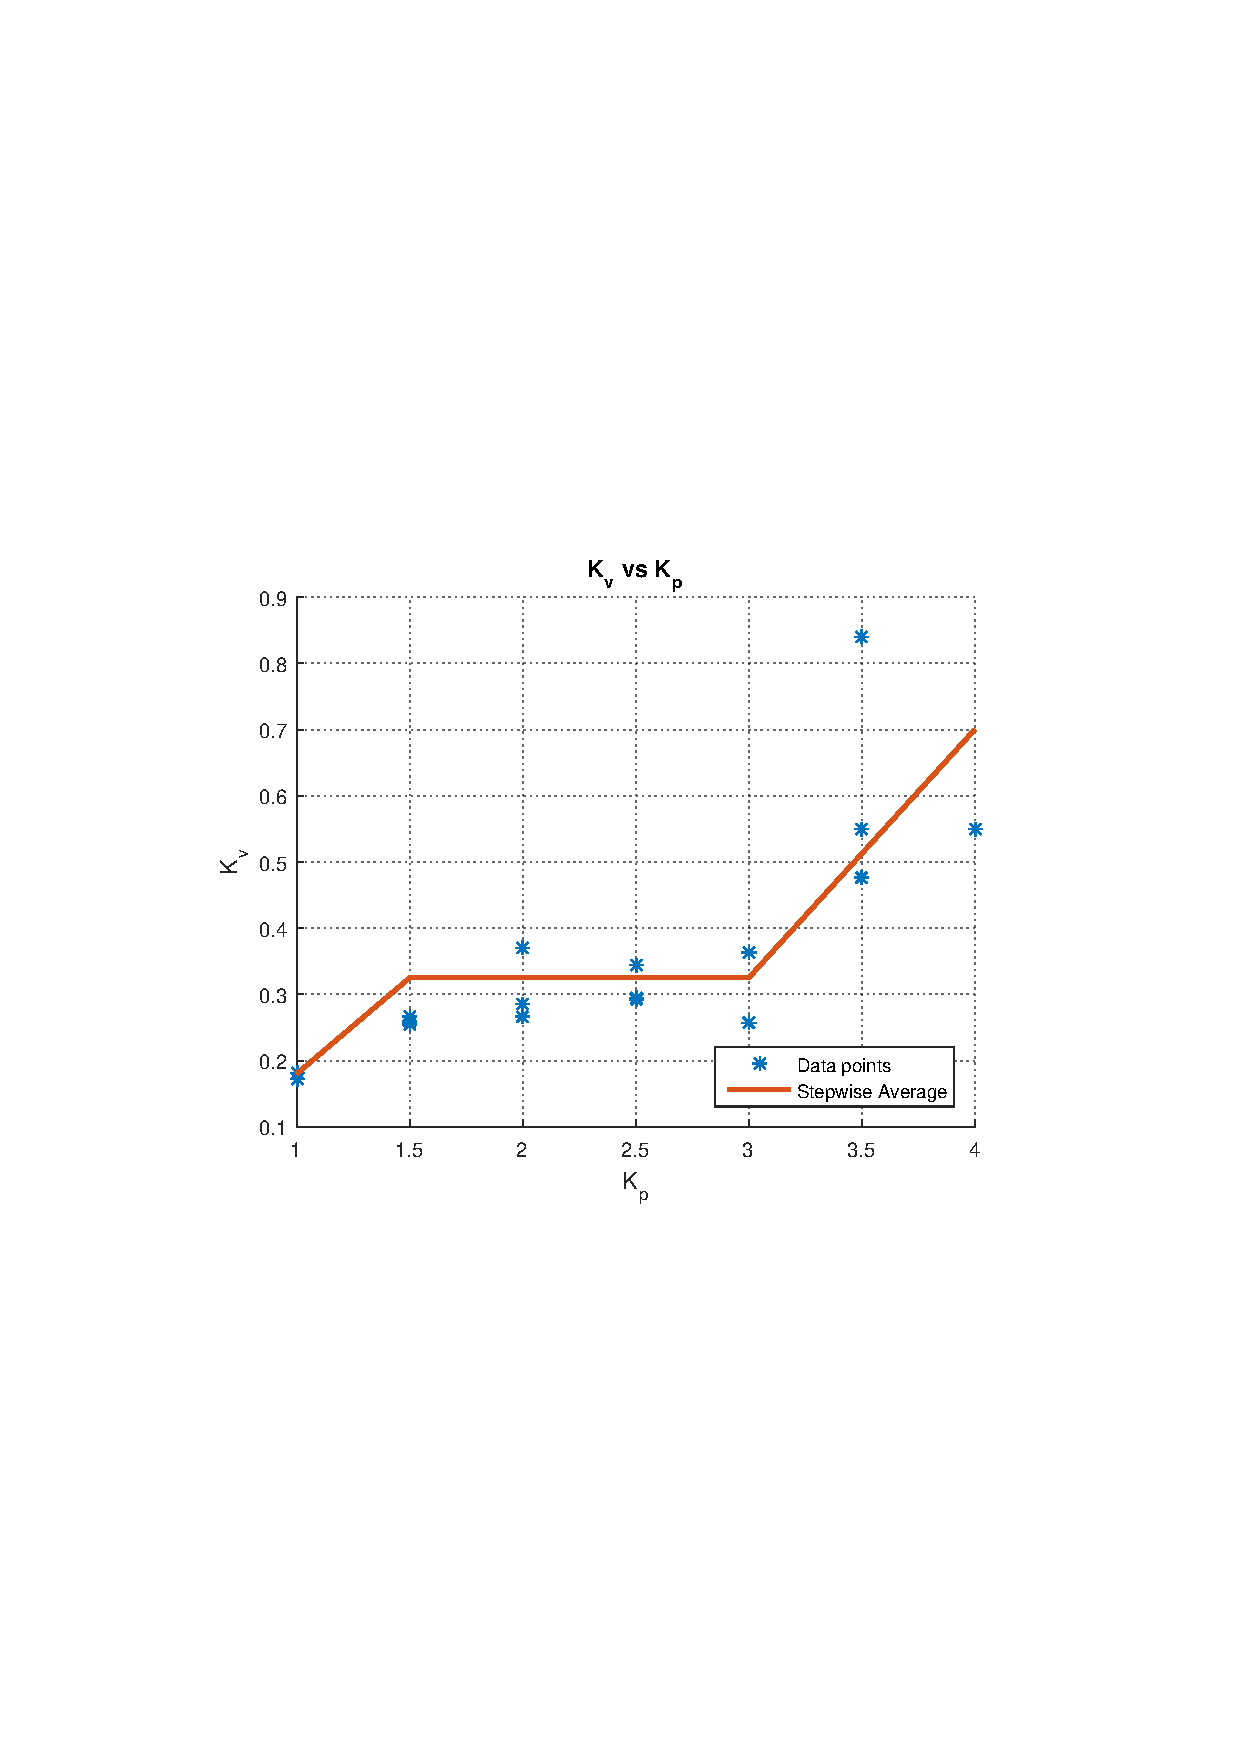
\includegraphics[width=1.2\textwidth]{figures/KvVsKp.pdf}
  }
  \caption{Plot of the gain \si{K_v} against the real speed.}
  \label{fig:steeringPlotKsteeringVsKp}
\end{figure}
%
The actual values from the test are plotted on \figref{fig:steeringPlotKsteeringVsKp}. It can be seen on this graph, that the steering gain is constant only for values of \si{K_p} from approximately \si{1,5} to \si{3}. The choice of a proportional controller gain should therefore account for this and stay within this linear area.